\paragraph{}
Comme nombre de projets, celui-ci est perfectible en différents points et nous avons listé les modifications qui seraient les plus intéressantes à réaliser par la suite.  

\paragraph{}
Au niveau de la prise de sons, il y a la possibilité d'améliorer celle-ci et d'obtenir plus de précision 
en implémentant un algorithme permettant de détecter les seuils à prendre en compte. Ceci permettrait une analyse beaucoup plus fine du son et ainsi une production de partitions plus fidèles à la réalité.

\paragraph{}
Au niveau de la sauvegarde des partitions, il serait possible de compresser un peu plus chaque fichier 
car il y a beaucoup d'espaces. Cela consisterait à améliorer le parser JSON des partitions. En effet, sur un petit fichier 
de 300 caractères, c'est-à-dire une partition de 2 accords comportant en tout 7 notes, le gain 
possible en enlevant les espaces est de 40\%. Ainsi, le remplissage de la base de données serait moins rapide, 
et les performances seraient également plus grandes.

\begin{figure}[H]
\centering
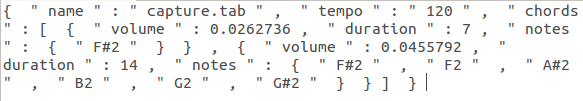
\includegraphics[scale=0.5]{FichierPartition}
\caption{Fichier representant une partition}
\end{figure}

\paragraph{}
Une grande amélioration serait également de rajouter la possibilité d'enregistrer plusieurs pistes. Cela permettrait donc de 
composer des musiques plus complètes avec par exemple une guitare rythmique et une guitare solo. Si l'on y ajoute également 
la possibilité de changer le son de l'instrument joué, cela permettrait de faire de ce projet une application de 
composition musicale vraiment très complète. En effet, cela permettrait d'ajouter exactement ce que l'on veut et ainsi 
avoir le rendu possible de la chanson finale.

\paragraph{}
Les données de connexion à la base de données sont enregistrées en clair dans un fichier de configuration, il faudrait changer 
ce fichier et le crypter pour que les utilisateurs ne puissent pas accéder à cette donnée confidentielle. Il faudrait également 
implémenter le même algorithme de hashage dans l'application que dans le serveur afin de sécuriser la connection de l'utilisateur 
par le biais de l'application. 

\paragraph{}
Une autre amélioration possible serait l'ajout de la possibilité pour l'utilisateur de consulter les partitions qu'il possède sur sur le site web et de les télécharger. Cette implémentation était déjà en court mais n'a pas pu être finalisée dans les délais.
De plus, on pourrait ajouter la possibilité de télécharger en une fois l'ensemble des partitions qu'il possède afin de lui faciliter cette tâche fastidieuse dans le cas où il veut importer toutes ses oeuvres sur un nouveau PC.

\paragraph{}
Afin de faciliter le déplacement lors de la lecture et de l'enregistrement de la partition, nous avions dans l'intention d'ajouter 
deux curseurs graphiques (l'un correspondant à la lecture et l'autre à l'enregistrement) afin de pouvoir réaliser les deux simultanément. Nous pourrions ainsi mettre sur pause à un endroit voulu, modifier les notes, faire revenir le curseur en arrière et 
écouter le résultat obtenu. Ces deux curseurs faciliteraient donc amplement les tâches de naviguation à travers les différentes parties de la partition. 
Si on joint ceci à la fonctionnalité d'avoir plusieurs pistes instrumentales, on pourrait placer le curseur de lecture à un endroit et le curseur 
d'enregistrement au même endroit, et ainsi jouer en même temps que ce que l'on synthétisela piste pré-existante.

\paragraph{}
On a préparé la possibilité d'implémenter l'utilisation de skins pour modifier l'apparence de l'application afin que le client puisse personnaliser son logiciel comme il le souhaite. Des emplacements de personnalisation sont déjà présents dans la fenêtre de configuration.\\
De plus, on aurait pu réserver une zone du site web pour y recenser tous les skins existants et permettre à l'utilisateur de télécharger celui qui lui plait. 
Il faudrait pour cela faire en sorte de pouvoir enregistrer le skin sous forme de fichier afin de le partager. 

\paragraph{}
Une autre option souhaitable pour l'utilisateur serait de pouvoir annoter et commenter des partitions, afin de clarifier la manière de la jouer.

\paragraph{}
Enfin une dernière amélioration serait de laisser à l'utilisateur de choisir lui-même l'entrée audio qu'il veut utiliser plutôt que de lui imposer l'entrée standard.
